% File example.tex
% Contact: simonnet@ecole.ensicaen.fr
%
% version 1.0 (July 24, 2009)
% version 1.1 (September 3, 2009)
% add using of the optional command: \secondauthoraddr



\documentclass[10pt]{article}

% File icdp2009.sty
% Preamble that you have to include to use the template  

% July 24, 2009
% Contact: simonnet@ecole.ensicaen.fr


\usepackage[a4paper,textwidth=18cm,textheight=24cm,top=2.85cm, bottom=2.85cm, left=1.5cm, right=1.5cm]{geometry}

\usepackage{template/icdp2009}

% left justified caption
\makeatletter
\long\def\@makecaption#1#2{%
\vskip\abovecaptionskip
\sbox\@tempboxa{#1. #2}%
\ifdim \wd\@tempboxa >\hsize
#1. #2\par
\else
\global \@minipagefalse
\hb@xt@\hsize{\box\@tempboxa\hfil}%
\fi
\vskip\belowcaptionskip}
\makeatother




%other package
\usepackage{amsmath}

% vectorial font
\usepackage{lmodern}

\usepackage{graphicx}
\usepackage{times}


\begin{document}
\noindent

\bibliographystyle{plain}

\title{Linear Regression\\Assignment 2 of Machine Learning I, 2022/2023}

\authorname{Mura Alessio}
\authoraddr{DIBRIS - Dipartimento di Informatica, Bioingegneria, Robotica e Ingegneria dei Sistemi\\
Università Degli Studi di Genova}

% \secondauthoraddr{+Affiliation,Country and contact details }


\maketitle

% % \keywords
% % Maximum 5 keywords placed before the abstract.

% \abstract
% This is where the abstract should be placed. It should consist
% of one paragraph and a concise summary of the material
% discussed in the article below. It is preferable not to use
% footnotes in the abstract or the title. The acknowledgement
% for funding organisations etc. is placed in a separate section at
% the end of the text. We wish you success with the preparation
% of your manuscript.

\section{Introduction}
Linear regression is an algorithm used to predict, or visualize, a relationship between two different features/variables. In linear regression tasks, there are two kinds of variables being examined: the dependent variable and the independent variable. \\\\The independent variable is the variable that stands by itself, not impacted by the other variable. As the independent variable is adjusted, the levels of the dependent variable will fluctuate. The dependent variable is the variable that is being studied, and it is what the regression model solves for/attempts to predict. In linear regression tasks, every observation/instance is comprised of both the dependent variable value and the independent variable value.\\\\ \textit{Linear} means that the
approximation uses a first order polynomial function to approximate the data. This implies that, in the case of a one-dimensional problem, the approximation will be a line.

\section{Theory of Linear Regression}
\subsection{One-dimensional problem}
Keeping in mind that the linear regression defines a linear approximation, the problem can be formalized in the following way:\\\\
Define a linear function such that, given an input \textit{x} (observation), computes the target \textit{t} that best approximates the real
value \textit{y}.
\begin{equation}
    t \approx y, where \rightarrow t = wx
\end{equation}
\textit{w} is the linear regression parameters, and associate with a linear function the input and the target.\\\\
Suppose there are two different observation $x_0$ and $x_1$.\\
Arranging the equation 1 it is simple to get the value of \textit{w}, which is:
\begin{equation}
    w_0 = \frac{x_0}{t_0}
\end{equation}
\\\\\\\\\\
However, with the second observation we get:
\begin{equation}
     w_0 = \frac{x_1}{t_1}
\end{equation}
It is clear that, comparing the equation 2 and 3, the two values of \textit{w}, \textit{$w_0$} and \textit{$w_1$}, can not be the same if the observation are
different, so we understand that the approximation can’t ever
be \textit{perfect}, and it introduces a small error to the target result.\\\\
Linear regression aims to compute the best value of \textit{w} that
better approximates every observation. \textit{w} must then minimize
the mean error.\\\\
Square error (SE) is then the best solution for finding the
best value of w, because it grows more than linearly, giving
heavier weight to larger errors. It is also even, meaning that $(y - t)^2 = (t - y)^2$
, and it is differentiable with respect to the
model output:
\begin{equation}
     \frac{d}{dx}\lambda_S_E\left(y,t\right)=2\left(y-t\right)
\end{equation}
Since we need to take the \textit{mean} SE, we can use the Mean Square error (MSE), that can be computed as:
\begin{equation}
     J_M_S_E=\frac{1}{N}\sum_{i=1}^{N}{\left(t_i - y_i\right)^{2}}
\end{equation}
After some computation, it is proven that the best value of
\textit{w} that approximates the best the value of the set of observation
is:
\begin{equation}
     w=\frac{\sum_{l=1}^{N}{x_l t_l}}{\sum_{l=1}^{N}{x_l}^2}
\end{equation}
With the equation 6 is then possible to get the best value
of \textit{w} for the equation 1.
\subsection{One-dimensional problem with intercept}
It is possible to build a better regression model using an
interception factor, $w_0$, that can move to the left or to the
right the approximation line, The equation 1 becomes then:
\begin{equation}
    t = w_0 x + w_1
\end{equation}
The two parameters, w0 and w1 can then be computed as follows:
\begin{equation}
     w_1=\frac{\sum_{l=1}^{N}{\left(x_l - \bar{x}\right)\left(t_l - \bar{t}\right)}}{\sum_{l=1}^{N}{\left(x_l - \bar{x}\right)}^2}
\end{equation}
\begin{equation}
    w_0 = \bar{t} - w_1 \bar{x}
\end{equation}
\subsection{Multi-dimensional problem}
The equations above can be generalized for the multidimensional case. Let \textbf{X} the set of observation, each of
them with multiple variables. Let \textbf{w} the vector of all the
approximation parameters, one for each variable, including $w_0$
intercept parameter:
\begin{equation}
    \textbf{X} =\begin{bmatrix}
            x_1\\
            x_2\\
            .\\
            .\\
            x_n\\
        \end{bmatrix} =
        \begin{bmatrix}
            x_1_,_1 & x_1_,_2 &.&.&x_1_,_n\\
            x_2_,_2 & x_2_,_2 &.&.&x_2_,_n\\
            .&.&.&.&.\\
            .&.&.&.&.\\
            x_n_,_n & x_n_,_2 &.&.&x_n_,_n\\
        \end{bmatrix}
\end{equation}
\begin{equation}
    \textbf{w} =\begin{bmatrix}
            w_0\\
            w_1\\
            w_2\\
            .\\
            .\\
            w_n\\
        \end{bmatrix} 
\end{equation}
The final output oh the linear regression will be:
\begin{equation}
    y_i = w_0 + x_i_,_1 w_1 + x_i_,_2 w_2 + ... + x_i_,_n w_n
\end{equation}
We then obtain:
\begin{equation}
    \textbf{y} =
        \begin{bmatrix}
            1&x_1_,_1 & x_1_,_2 &.&.&x_1_,_n\\
            1&x_2_,_1 & x_2_,_2 &.&.&x_2_,_n\\
            .&.&.&.&.\\
            .&.&.&.&.\\
            1&x_n_,_1 & x_n_,_2 &.&.&x_n_,_n\\
        \end{bmatrix}
        \begin{bmatrix}
            w_0\\
            w_1\\
            w_2\\
            .\\
            .\\
            w_n\\
        \end{bmatrix} = \textbf{X}\textbf{w}
\end{equation}
Note that a constant column of ones is added in the first matrix,
in order to incorporate $w_0$.\\\\
As for the one-dimensional case, also here it is necessary to minimize the MSE. Since we are dealing with matrices and not one-dimensional variables, now we must set $\nabla J_M_S_E = 0$. We can then find \textbf{w} as follows:
\begin{equation}
\textbf{w}=\left(\textbf{X}^T\textbf{X}\right)^{-1} \textbf{X}^T\textbf{t} = \textbf{X}^{\dagger}\textbf{t}
\end{equation}
Where $\textbf{X}^{\dagger}$
is the Moore-Penrose pseudoinverse of \textbf{X}. Notice
that computing the pseudoinverse can result in introducing a
small but notable error in the calculation. This small error
however can be quickly amplified by the condition number
and cause large errors on the result.

\section{THE ASSIGNMENT}
The given assignment consist of three tasks:
\begin{itemize}
 \item \textbf{Task 1}: Get data
 \item \textbf{Task 2}: Fit a linear regression model
 \item \textbf{Task 3}: Test regression model
 \end{itemize} 

\subsection{Task 1: Get data}
This assignment takes into account two different sets:
\begin{itemize}
 \item turkish-se-SP500vsMSCI (Turkish stock exchange data);
 \item mtcarsdata-4features (1974 Motor Trend Car Road Tests).
 \end{itemize}
 The first set is composed by 536 observations and 1 variable. The second set is composed by 32 observations and 3
variables.\\\\The Two sets are initially stored as .csv files. To import
them in Python it is required to use the function read-csv(), inside Pandas library, in order to store them into dataframes.

\subsection{Task 2: Fit a linear regression model}
In the second tasks, we have to compute the linear regression parameters in four different cases:
\begin{enumerate}
    \item One-dimensional problem without intercept on the Turkish stock exchange data;
    \item Compare graphically the solution obtained on different random subsets (10\%) of the whole data set;
    \item One-dimensional problem with intercept on the Motor Trends car data, using columns mpg and weight;
    \item Multi-dimensional problem on the complete MTcars data, using all four columns (predict mpg with the other three columns).
\end{enumerate}
\subsubsection{1}
In order to compute and visualize the linear regression, we created a function, \textit{BuildGraph()}, in which we passed: the turkish dataset, the two columns, and a boolean value, which could be \textit{yes} [TRUE] or \textit{no} [FALSE].\\\\
In this case, we passed \textit{yes}, meaning that we want to compute the linear regression without intercept. In fact, inside \textit{BuildGraph()}, after creating a vector with the the variables we need by \textit{create-vector()} function and thanks to the boolean value yes, we call three functions: \textit{estimate-coef-without-intercept()}, \textit{OneDimensionalMeanSquareError()} and \textit{plot-regression-line-with-intercept()}.
\\\\
By these functions, we estimated the \textit{w} coefficient without intercept, we computed the mean square error and, finally, we plotted the result into a graph. All these steps have been done following the theory explained in the \textit{Theory of Linear Regression} section.
\subsubsection{2}
In order to get different subsets with 10\% of the whole data, we created a function, \textit{randomSubset()}, where we compute the linear regression without intercept in the same way as the previous step. The final results will be shown in a subplot.
\subsubsection{3}
In order to compute the linear regression with intercept on MotorTrendsCar dataset, we reused \textit{BuildGraph()} function, but, this time, the boolean value is \textit{no}, in order to compute it taking into account of intercept.
By computing it, we used mpg and weight columns.
\subsubsection{4}
In this last step, we created a new function, \textit{MultiDimensional()}, in order to predict \textit{mpg} with the other three columns. Obviously, the dataset we used is MotorTrendsCar.
According with the theory, we compute the mean square error for the multi-dimensional case by \textit{MultiDimensionalMeanSquareError()} function and, finally, printed our prediction.


\subsection{Task 3: Test regression model}
The last task requires to re-run 1,3 and 4 from task 2 using only 5\% of the data, compute the objective (mean square error) on the training data, compute the objective of the same models on the remaining 95\% of the data and repeat for different training-test random splits.

\section{RESULTS}

\begin{figure}[h] 
	\centering
	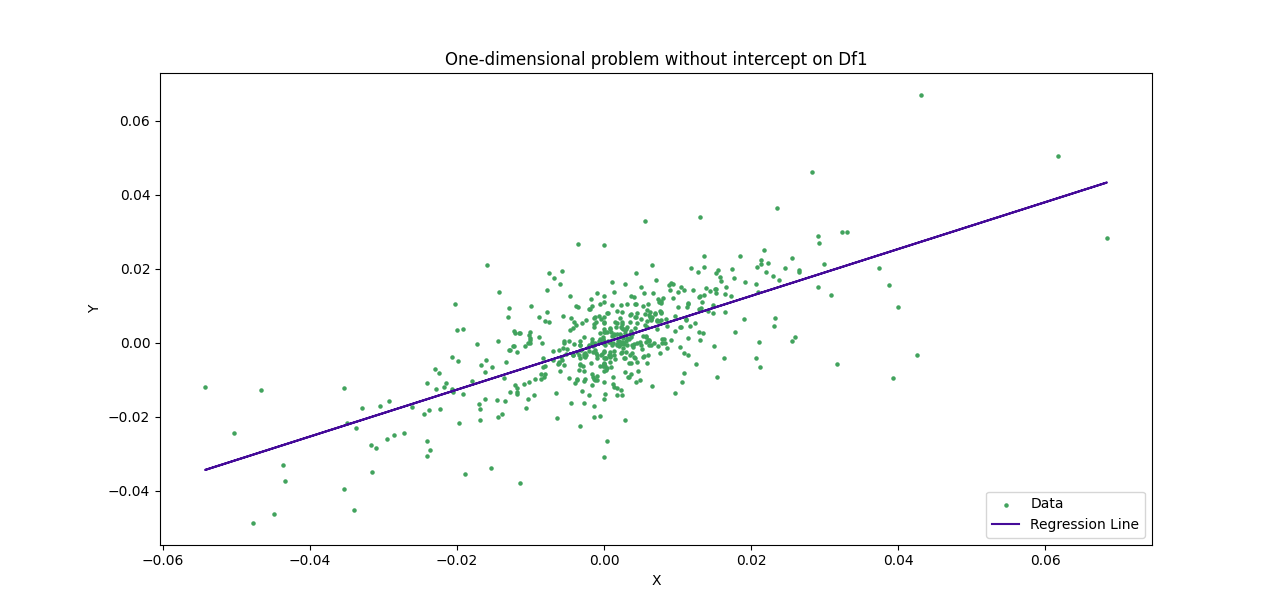
\includegraphics[width=0.9\columnwidth]{Figure_1.png} % Example image
	\caption{One-dimensional problem without intercept.}
\end{figure}


As we can clearly see in Figure 1, we found the best value of \textit{w} that approximates our observation. The fact that we did not use the intercept is denoted by the passage of the regression line through the origin.
\begin{figure}[h] 
	\centering
	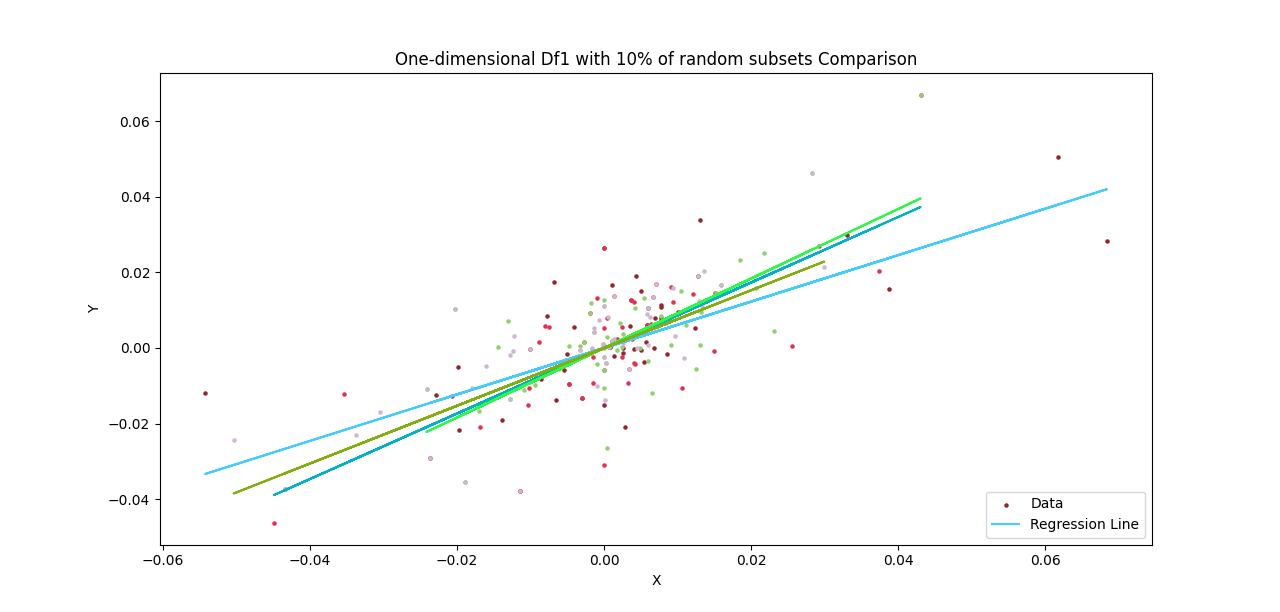
\includegraphics[width=0.9\columnwidth]{Figure_2.png} % Example image
	\caption{One-dimensional problem without intercept with random subsets using 10\% of the whole data.}
\end{figure}
\newpage
The figure 2 shows instead a graphically comparison between different random subsets (10\%) of the whole data set. we can observe that all the graphs are similar to each other and also similar to the result obtained using the whole dataset.

\begin{figure}[h] 
	\centering
	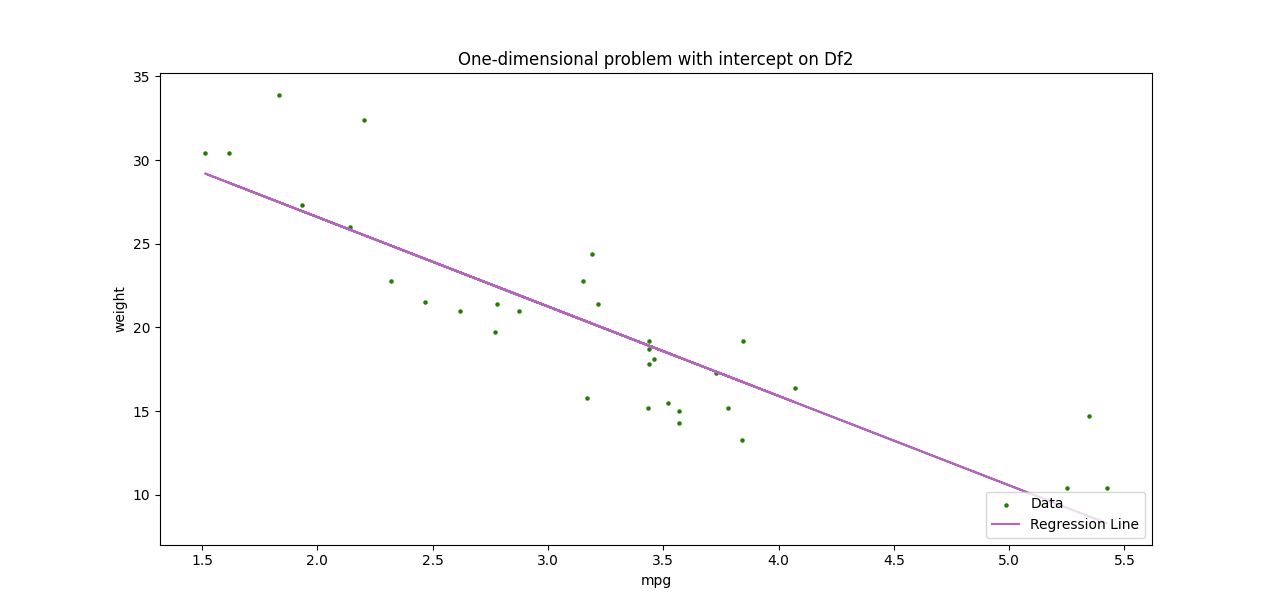
\includegraphics[width=1.0\columnwidth]{Figure_3.png} % Example image
	\caption{One-dimensional problem with intercept.}
\end{figure}



In the figure 3 we can see the linear regression with the intercept factor. This is still a one-dimensional problem: only the car weight is used as variable. In this case, the dataset we used is MotorTrendsCar.


\begin{figure}[h] 
	\centering
	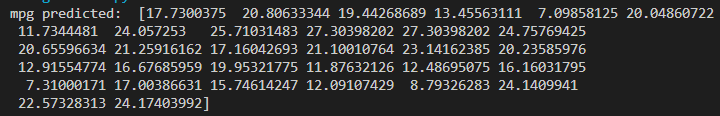
\includegraphics[width=1.0\columnwidth]{mpg.png} % Example image
	\caption{mpg prediction using the Multi-dimensional regression}
\end{figure}
By Figure 4, It is clearly visible that our mpg prediction, using the multi-dimensional linear regression on MotorTrendsCar dataset, is quite successful. The prediction we obtained is similar to the real values of mpg. Obviously our prediction is affected by error.
\newpage

\begin{figure}[h] 
	\centering
	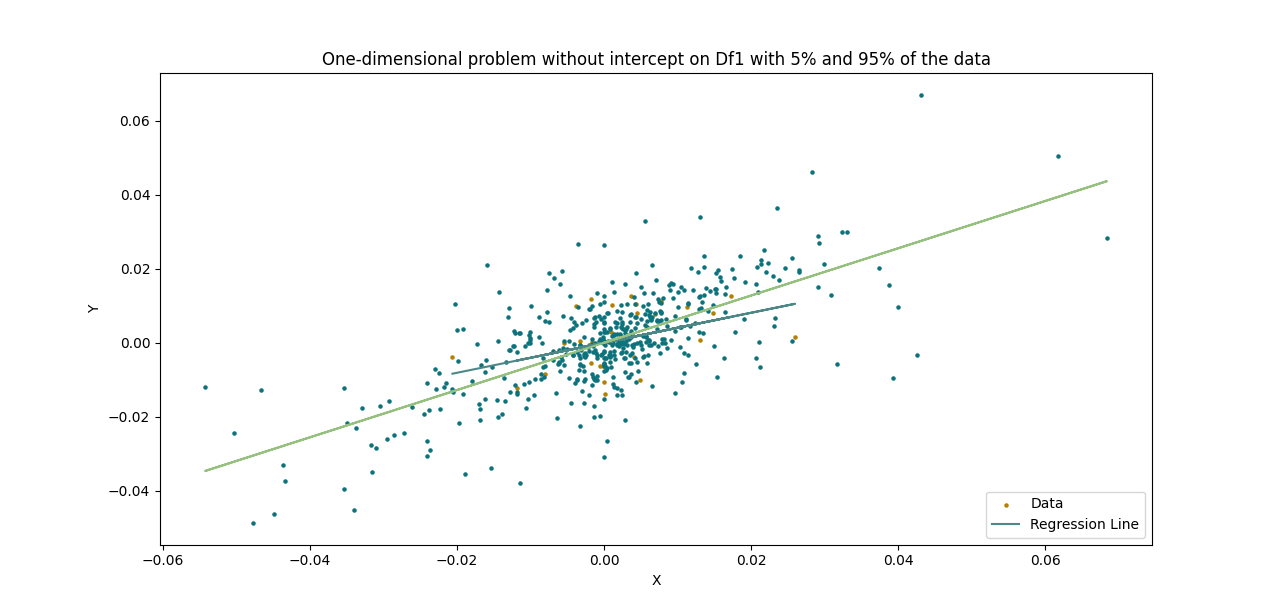
\includegraphics[width=1.0\columnwidth]{Figure_4.png} % Example image
	\caption{One-dimensional problem without intercept using 5\% and 95\% of the data.}
\end{figure}


As in Figure 1, in Figure 5 we found the best value of \textit{w} that approximates our observation by using 5\% and 95\% of the whole dataset. They are quite similar to each other and to the result using the whole dataset: also the slops of the regression lines are similar.
\begin{figure}[h] 
	\centering
	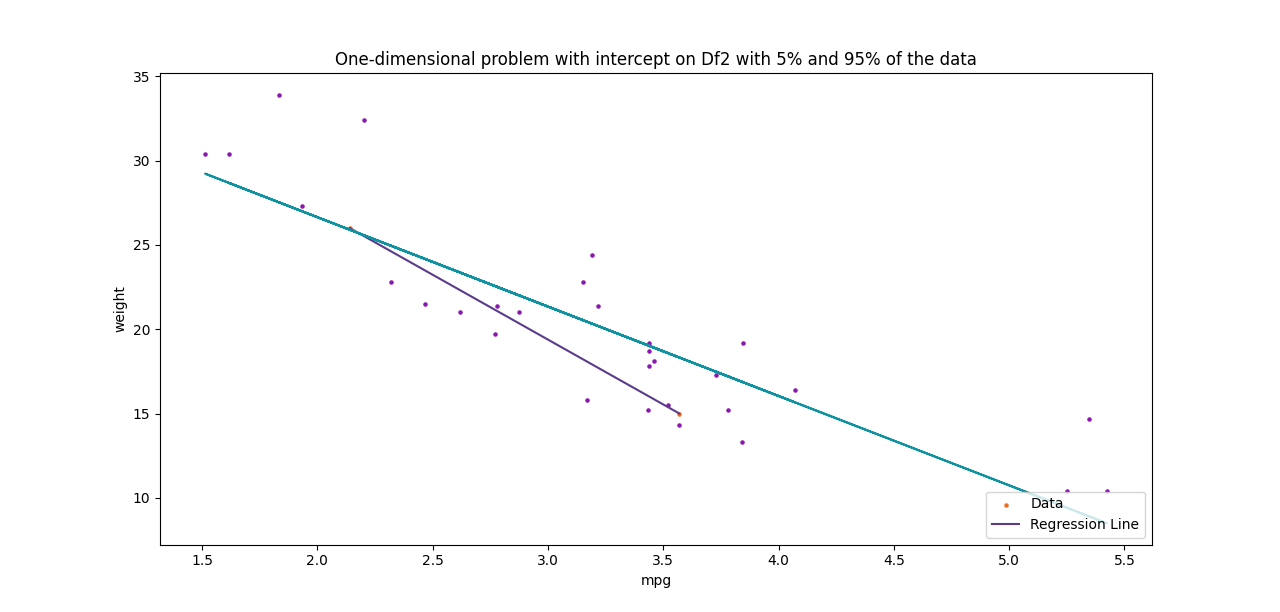
\includegraphics[width=1.0\columnwidth]{Figure_5.png} % Example image
	\caption{One-dimensional problem without intercept using 5\% and 95\% of the data.}
\end{figure}

As in Figure 3, in Figure 6 we can see the linear regression with the intercept factor by using 5\% and 95\% of the whole dataset. If the subset should correspond to the 5\% of the total set,
it means that the cars data set should be composed
by only 2 observations. This has some consequences on the
test outcome: If a set is made of only two observation, the
computed factor \textit{w} will then be perfect. As a proof, consider
that \textit{w} is the slope of the correspondent regression line. Given only two points, there’s one and only one line that passes
through them, and that line matches the regression line. In this case $J_M_S_E = 0$.


\begin{figure}[h] 
	\centering
	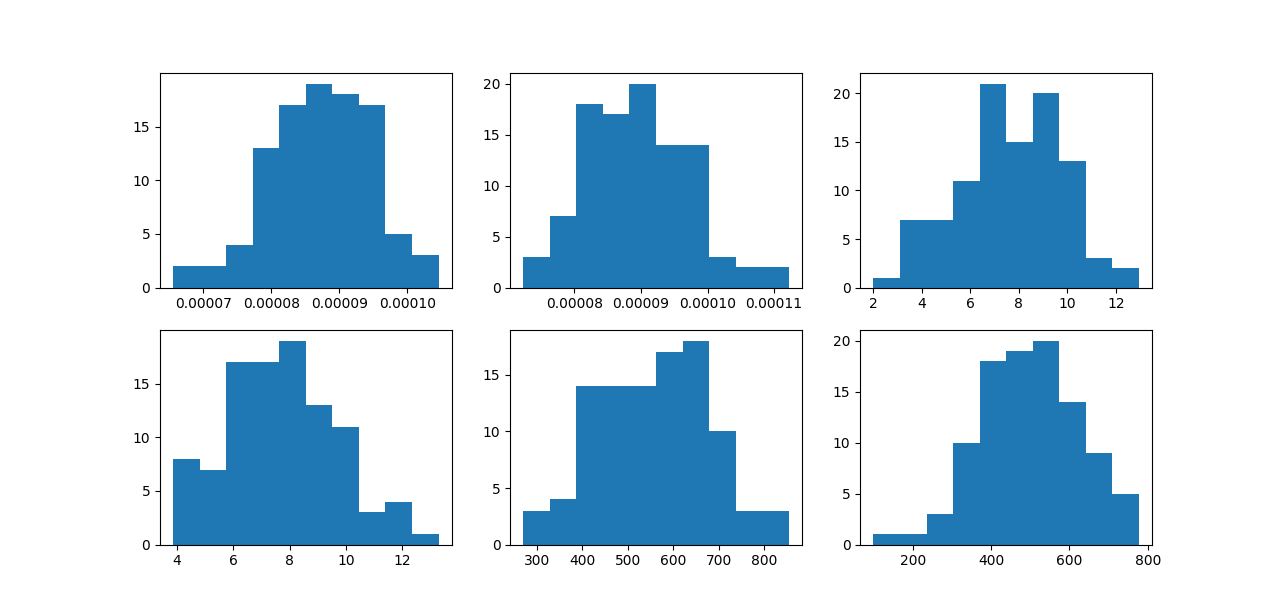
\includegraphics[width=1.0\columnwidth]{Figure_6.png} % Example image
	\caption{Hist of different training-test random splits.}
\end{figure}

The figures 7 shows a comparison of the computed objectives obtained with 100 random \% of subsets, and the objectives of their consequent remaining subsets. \\\\We created a subset of histograms for every case: first column for One-dimensional problem on Turkish dataset, second column for One-dimensional problem on  MotorTrendscar dataset and the third column for Multi-dimensional problem MotorTrendscar dataset.
\\\\We can infer that our analysis has been successful by the fact that our histograms present a bell-shaped graphs.

\end{document}